\chapter{{\LaTeX}\ Specific Usage}

This template is heavily built on \href{https://www.ctan.org/pkg/memoir}{memoir} package.
It's recommended to also check out memoir's documentation for its detailed usage and available customizations.


\section{Figures}
Common file formats (PDF, PNG, and JPG) are supported.
Vector figures should be stored as PDF files to prevent pixelation.
For example, \fref{fig:vector} is a vector figure.

\begin{figure}[tbh]
  \centering
  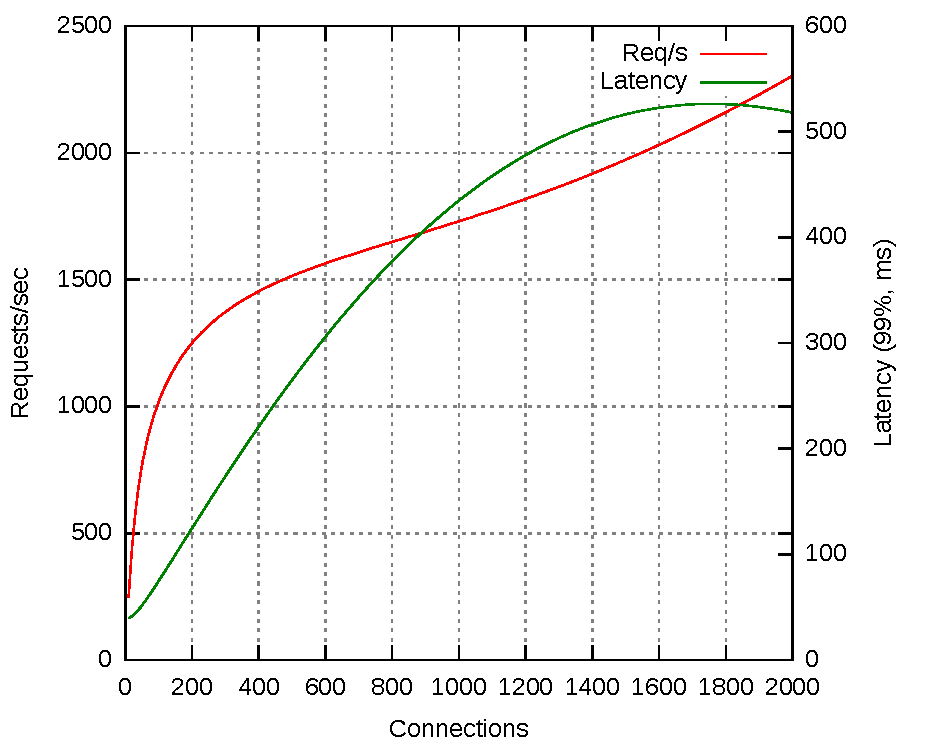
\includegraphics[width=0.6\textwidth]{figures/just-a-plot}
  \caption{Example vector figure in PDF.}
  \label{fig:vector}
\end{figure}



\section{Subfigures and subtables}
If a figure has multiple panels (subfigures), use \texttt{subcaption} package to enable the correct references for subfigures.
Use \cmd{\fref}\marg{labstr} to refer to the full figure and \cmd{\fref}\marg{sublabstr} to refer to a specfic panel of that figure.
Use \cmd{\subcaptionref}\marg{sublabstr} to refer to just the panel number.
For example, \fref{fig:subfigure-demo} has two panels, \subcaptionref{fig:subfigdemo-cat} and \subcaptionref{fig:subfigdemo-dog}.
This example manually specified the panel numbering since it is often to have figures with the panel numbers embedded.
\fref{fig:subfigdemo-cat} refers to the cat panel.

\begin{figure}[t]
    \begin{subfigure}[b]{.5\linewidth}
        \centering
        \textbf{\sffamily A}\\[-0.5\onelineskip]
        \HUGE Cat \\
        \emoji{cat} \emoji{cat-face}
        \phantomsubcaption\label{fig:subfigdemo-cat}
    \end{subfigure}%
    \begin{subfigure}[b]{.5\linewidth}
        \centering
        \textbf{\sffamily B}\\[-0.5\onelineskip]
        \HUGE Dog \\
        \emoji{dog} \emoji{dog-face}
        \phantomsubcaption\label{fig:subfigdemo-dog}
    \end{subfigure}
    \caption{Two animals and their emojis. \subref{fig:subfigdemo-cat} cats
    and \subref{fig:subfigdemo-dog} dogs.}
    \label{fig:subfigure-demo}
\end{figure}

Similarly, multiple tables can be grouped together as one using the same method. For example, see \tref{tab:subtable-demo}, which has two panels \subcaptionref{tab:subtab-a} and \subcaptionref{tab:subtab-b}.

\begin{table}[b]
    \centering
    \caption{Another table with two panels: \subref{tab:subtab-a} first and \subref{tab:subtab-b} second panel}
    \label{tab:subtable-demo}

    \begin{subtable}{0.5\linewidth}
        \centering
        \subcaption{First}\label{tab:subtab-a}
        \begin{tabular}{lc} \toprule
        A legendary table & 5 \\
        with two lines    & 6 \\ \bottomrule
        \end{tabular}
    \end{subtable}%
    \begin{subtable}{0.5\linewidth}
        \centering
        \subcaption{Second}\label{tab:subtab-b}
        \begin{tabular}{lc} \toprule
        A legendary table & 5 \\
        with two lines    & 6 \\ \bottomrule
        \end{tabular}
    \end{subtable}
\end{table}


\subsection{Merged figure with multiple panels}





\section{Citations}
This paper demonstrated CRISPR can cut DNA at specific nucleotide sequences \cite{Jinek2012}.


\section{Equations}
See Equation~\ref{eq:maxwell}.

\begin{equation}
    \label{eq:maxwell}
    \begin{aligned}
    \frac{\partial\mathcal{D}}{\partial t} & = \nabla\times\mathcal{H},   & \text{(Loi de Faraday)}\\
    \frac{\partial\mathcal{B}}{\partial t} & = -\nabla\times\mathcal{E},  & \text{(Loi d'Ampère)}\\
    \nabla\cdot\mathcal{B}                 & = 0,                         & \text{(Loi de Gauss)}\\
    \nabla\cdot\mathcal{D}                 & = 0.                         & \text{(Loi de Colomb)}
    \end{aligned}
\end{equation}

\clearpage
\section{Page layout}
\layout
